\documentclass[a4paper]{article}
\usepackage[spanish]{babel}
\spanishdecimal{.}
\selectlanguage{spanish}
\usepackage[spanish,onelanguage,ruled]{algorithm2e}
\usepackage[utf8]{inputenc}
\usepackage{graphicx}
\usepackage{caption}
\usepackage{subcaption}
\usepackage[top=2.5cm, bottom=2.5cm, left=2.5cm, right=2.5cm]{geometry}
\usepackage{hyperref}
\usepackage{verbatim}
\usepackage{amssymb}
\usepackage{mathtools}
\usepackage{gensymb}
\usepackage[natbibapa]{apacite}
\bibliographystyle{apacite}
\newcommand\ddfrac[2]{\frac{\displaystyle #1}{\displaystyle #2}}
\DeclareMathOperator{\atantwo}{atan2}

\title{Robots Móviles y Agentes Inteligentes}
\author{M.I. Marco Negrete}
\date{Resumen de temas}
\begin{document}
\renewcommand{\tablename}{Tabla}
\maketitle

\tableofcontents

%%%%%
%%%%%INTRODUCCIÓN
%%%%%
\section{Introducción}

La palabra \textit{robot} tiene su origen en la obra \textit{Rossum's Universal Robots} del escritor checo $Karel \,\check{C}apeck$, publicada en 1921, y su significado es ``trabajo duro''. Existen varias definiciones de robot y en general varían dependiendo del campo de aplicación o del área de investigación. 

De acuerdo con la Real Academia Española, un robot es una máquina o ingenio electrónico programable capaz de manipular objetos y realizar operaciones antes reservadas sólo a las personas. Esta definición incluye conceptos como ``proglamable'' y ``manipulación de objetos'', sin embargo, no es la más adecuada para el tipo de robots que se desarrollarán en este curso. 

\cite{Latombe1991MotionPlanning} define un robot como un dispositivo mecánico versátil equipado con sensores y actuadores bajo el control de un sistema de cómputo. Dado que el objetivo de este curso es brindar cierto nivel de autonomía a un robot móvil, la definición más adecuada es la de \cite{Arkin1998BehBasedRobo}, quien propone que un robot inteligente es una máquina capaz de extraer información de su ambiente y usar el conocimiento acerca de su mundo para moverse de manera segura y significativa, con un propósito específico. Esta última definición es la más adecuada para los propósitos de este curso. 

En las secciones subsecuentes se tocarán temas últiles para brindar autonomía a un robot móvil, pero, ¿qué es un robot autónomo?. De acuerdo con \cite{Latombe1991MotionPlanning}, un robot autónomo es aquel que sólo necesita descripciones de alto nivel para llevar a cabo una determinada tarea y que no requiere de intervención humana para tal fin, es decir, las descripciones de entrada deberán especificar más el qué que el cómo. En este curso se abordará sólo el tema de la navegación autónoma. 

\subsection{Primitivas de la robótica}
Las tareas que puede llevar a cabo un robot pueden clasificarse en tres grandes conjuntos conocidos como primitivas de la robótica: sensar, planear y actuar. 

\textbf{Sensar:} Se refiere a la extracción de información ya sea del ambiente externo o interno del robot. 

\textbf{Planear:} Es la generación de subtareas y toma de decisiones a partir de la información obtenida de los sensores y/o de alguna representación del conocimiento generada anteriormente. La planeación genera \textit{directivas}.

\textbf{Actuar:} Es la modificación del ambiente por alguno de los dispositivos del robot. Los comandos enviados a los \textit{actuadores} del robot se generan a partir de la información sensada o de las directivas generadas por la planeación. 

Como se verá más adelante, la forma en que se relacionan las diferentes primitivas define los diferentes \textit{paradigmas de la robótica}.

\subsection{Componentes básicos de un robot móvil}
Cada una de las primitivas tiene un correlato en hardware: sensores, microcomputadoras y actuadores. 

\textbf{Sensores:} Son los transductores utilizados para extraer información del ambiente. Se pueden clasificar en propioceptivos o exteroceptivos dependiendo de si extraen información del ambiente interno o externo del robot respectivamente. Los encoders para los motores o los medidores de nivel de bateria son ejemplos de sensores propioceptivos mientras que las cámaras y micrófonos son ejemplos de sensores exteroceptivos. 

Otra forma de clasificar los sensores es en activos y pasivos. Los primeros son aquellos que necesitan emitir energía para realizar el sensado, contrario a los segundos, que no requieren de dicha emisión. Ejemplos de sensores pasivos son las cámaras RGB, micrófonos o sensores de contacto. Una cámara infrarroja o un sensor láser son ejemplos de sensores activos. 

\textbf{Microcomputadoras:} En esta categoría entran los CPUs, GPUs, microprocesadores, microcontroladores, DSPs, etc. La elección de alguno de estos está en función del tipo de procesamiento que se desee realizar.

\textbf{Actuadores:} Son los dispositivos que sirven para realizar alguna modificación al ambiente. En el caso de los robots móviles autónomos, los más utilizados son los eléctricos. 

\subsection{Paradigmas de la robótica}
Los paradigmas de la robótica se definen en función de la forma en que se relacionan las primitivas y existen tres: el jerárquico o tradicional, el reactivo y el híbrido. 

\textbf{Jerárquico:} En este paradigma las tres primitivas se realizan en forma secuencial, como se muestra en la figura  \ref{fig:ParadigmHierarchical}. Tiene las siguientes características:
\begin{figure}
  \centering
  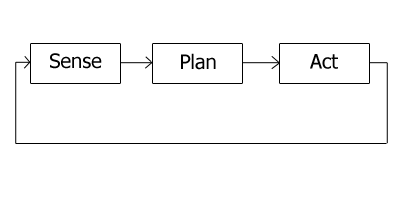
\includegraphics[width=0.5\textwidth]{Figures/Hierarchical.png}
  \caption{Paradigma jerárquico o tradicional.}
  \label{fig:ParadigmHierarchical}
\end{figure}
\begin{itemize}
\item Fuerte dependencia de una representación interna del ambiente. 
\item El tiempo de respuesta es lento comparado con el paradigma reactivo. 
\item El costo computacional es alto.
\item Con este paradigma se pueden resolver tareas con algo nivel cognitivo.
\item Dada la dependencia de una representación del ambiente, la capacidad de predicción es alta.
\end{itemize}

\textbf{Reactivo:} En este paradigma el sensado y la actuación se conectan directamente sin que haya de por medio una planeación, como se muestra en la figura \ref{fig:ParadigmReactive}. Sus características en general son contrarias a las del paradigma jerárquico:
\begin{figure}
  \centering
  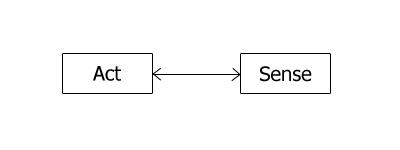
\includegraphics[width=0.5\textwidth]{Figures/Reactive.png}
  \caption{Diagrama de bloques del paradigma reactivo. }
  \label{fig:ParadigmReactive}
\end{figure}
\begin{itemize}
\item No requiere de una representación del ambiente.
\item El tiempo de respuesta es rápido comparado con el paradigma jerárquico.
\item Bajo costo computacional.
\item En general no es posible resolver tareas que requieran de un alto nivel cognitivo.
\item La capacidad de predicción es baja. 
\end{itemize}

\textbf{Híbrido:} Tiene como objetivo utilizar las ventajas de ambos paradigmas, es decir, emplear comportamientos reactivos para que el robot responda rápidamente ante cambios en el ambiente sin perder la alta capacidad cognitiva y de predicción que brinda el paradigma jerárquico. La figura \ref{fig:ParadigmHybrid} muestra la forma en que se relacionan las primitivas en este paradigma. 
\begin{figure}
  \centering
  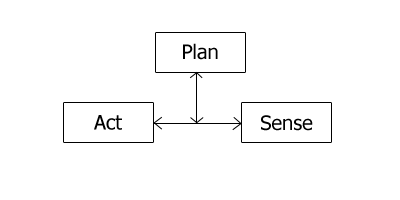
\includegraphics[width=0.5\textwidth]{Figures/Hybrid.png}
  \caption{Diagrama de bloques del paradigma híbrido.}
  \label{fig:ParadigmHybrid}
\end{figure}


%%%%%
%%%%%EL PROBLEMA DE LA PLANEACIÓN DE MOVIMIENTOS
%%%%%
\section{El problema de la planeación de movimientos}
\subsection{Tareas en la planeación de movimientos}
\label{sec:Tasks}

El problema de la planeación de movimientos comprende cuatro tareas principalmente: navegación, cobertura, localización y mapeo. 
Para estas cuatro tareas es necesario tener una descripción o representación de los puntos en el espacio que ocupa el robot. A esta descripción se le llama \textit{configuración} y el \textit{espacio de configuraciones} es el conjunto de todas las configuraciones posibles que puede tener el robot.

La navegación es el problema de encontrar un movimiento libre de colisiones desde una configuración inicial a una final. La cobertura se refiere al problema de mover un sensor o una herramienta de modo que se asegure que se cubren todos los puntos de un espacio determinado. La localización consiste en determinar la configuración del robot dado un mapa y un conjunto de lecturas de los sensores. El mapeo consiste en la exploración y sensado de un ambiente desconocido de modo que se obtenga una representación de dicho ambiente que sea últil para alguna de las otras tareas. Al problema de la localización y mapeo simultáneos se le conoce como SLAM (por sus siglas en inglés). 

En este curso se abordarán únicamente las tareas de navegación y localización. 

\subsection{Características del robot}
Para poder construir un planeador de movimientos es necesario conocer primero las características del robot a utilizar. La primera de ellas es el número de \textit{grados de libertad} que se refiere al número de parámetros independientes que definen la configuración del robot. En el caso de un robot móvil que sólo se mueve en el plano se tienen tres grados de libertad: dos coordenadas de posición $(x,y)$ y una orientación $\theta$. Los espacios de configuración pueden describirse empleando variedades y los grados de libertad definen la \textit{forma} de dicha variedad.

Otra característica importante son las restricciones de movimiento. Si el robot se puede mover en cualquier dirección en el espacio de configuración (en ausencia de obstáculos) se habla de un robot omnidirecciones. Si existen restricciones de velocidad, como en el caso de un automóvil que sólo se puede desplazar en la dirección en la que apuntan las llantas delanteras, entonces se habla de un robot con restricciones \textit{no holonómicas}. Es importante aclarar que una restricción es no holonómica cuando sólo se puede representar en términos de velocidades pero no de posición, por ejemplo, un robot diferencial sólo se puede mover con una velocidad perpendicular al eje que une las llantas, sin embargo, con la planeación adecuada, es posible alcanzar cualquier configuración. El caso contrario es la restricción de movimiento al plano $XY$ que se puede expresar como $\dot{z}=0$ (en términos de la velocidad) o como $z=Cte$ (en términos de la posición).

Finalmente, es importante tomar en cuenta si el modelo del robot será dinámico o solamente cinemático. En el primer caso las señales de entrada pueden ser fuerzas o pares y en el segundo se asume que las velocidades se pueden manipular arbitrariamente y por lo tanto pueden considerarse como señales de entrada. 

\subsection{Características de los algoritmos}

Una vez que se ha definido la tarea a realizar y con base en las características del robot, puede elegirse un algoritmo para resolver determinado problema. Si lo que nos interesa es que el robot ejecute una terea en un tiempo mínimo, con el menor gasto de energía posible o recorriendo la distancia más corta, entonces se requiere de un algoritmo \textit{óptimo}. 

El \textit{costo computacional} de un algoritmo se refiere a la cantidad de recursos necesarios para resolverlo, es decir, cantidad de memoria y tiempo de ejecución. La complejidad se expresa como función de la cantidad de datos de entrada y se suele clasificar como exponencial, polinomial, logarítmica, factorial, etc, dependiendo de la función que pueda acotar ya sea el peor caso o un promedio de los distintos casos. Los datos de entrada pueden ser el número de grados de libertad o el número de estados en un planeador, por ejemplo. 

Otra característica importante de los algoritmos es su \textit{completitud} (se empleará esta palabra a falta de una mejor traducción del vocablo \textit{completeness} en inglés). Se dice que un algoritmo es completo si garantiza encontrar la solución al problema si es que ésta existe. Algunas veces, para disminuir la complejidad de un algoritmo se maneja una completitud para una resolución dada, es decir, el algoritmo garantiza encontrar una solución si se maneja un cierto nivel de discretización. Un ejemplo de esto se verá en la sección \ref{sec:AStar}, en el que una ruta se puede calcular sólo si el espacio navegable se discretiza. 

Una última característica que está más relacionada con la implementación del planeador que con los algoritmos en general, es aquella que se refiere al momento en que se realiza la planeación. Si el planeador construye un plan previo a la ejecución se dice que éste es \textit{fuera de línea}. Si el planeador actualiza el plan conforme lo ejecuta, entonces se dice que es \textit{en línea}.

%%%%%
%%%%% PLANEACIÓN DE RUTAS
%%%%%
\section{Planeación de rutas}
\label{sec:PathPlanning}
\subsection{Celdas de ocupación}

El primer paso para resolver la tarea de navegación es la planeación de una ruta con base en un mapa construido previamente. Como se mencionó en la sección \ref{sec:Tasks}, un mapa es una representación del ambiente que contiene información útil para tomar decisiones. En este curso se emplerán mapas basados en \textit{celdas de ocupación}. En esta representación, el espacio se discretiza con una resolución determinada y a cada celda se le asigna un número $p\in[0,1]$ que indica su nivel de ocupación. En un enfoque probabilístico este número se puede interpretar como la certeza que se tiene de que una celda esté ocupada. 
\begin{figure}
  \centering
  \begin{subfigure}{0.4\textwidth}
    \centering
    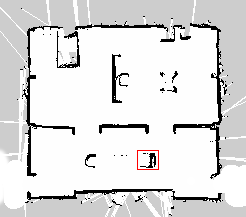
\includegraphics[width=0.8\textwidth]{Figures/OccupancyGrid.png}
    \caption{A pesar de ser una discretización, con una buena resolución la representación puede ser bastante exacta. Este es un mapa obtenido con el Robot Justina.}
  \end{subfigure}
  \hspace{0.05\textwidth}
  \begin{subfigure}{0.4\textwidth}
    \centering
    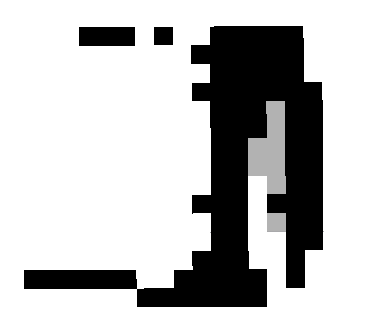
\includegraphics[width=0.8\textwidth]{Figures/UniversumZoom.png}
    \caption{Parte del mapa ampliada donde se aprecia la discretización: las partes blancas son celdas libres, las negras, ocupadas y las grises, aquellas sin información.}
  \end{subfigure}
  \caption{Ejemplos de celdas de ocupación.}
  \label{fig:OccGrids}
\end{figure}

\subsection{El algoritmo A*}
\label{sec:AStar}
Si se tiene un mapa del ambiente con celdas de ocupación, el problema de la planeación de rutas se puede resolver aplicando un algoritmo de búsqueda en grafos. En este caso cada celda representa un nodo en el grafo y se considera que está conectada únicamente con aquellas celdas vecinas que pertenezcan al espacio libre. Para determinar los nodos vecinos se puede utilizar conectividad cuatro u ocho.

A* es un algoritmo de búsqueda que explora la ruta con el menor costo esperado. Para un nodo $n$, el costo esperado $f(n)$ se calcula como 
\[f(n) = g(n) + h(n)\]
donde $g(n)$ es el costo de la ruta desde el nodo origen hasta el nodo $n$ y $h(n)$ es una heurística que determina \textit{un} costo que se esperaría tener desde el mismo nodo $n$ hasta el nodo objetivo. Este costo esperado de hecho subestima el valor real, es decir, se debe cumplir que $h(n) \leq g(n)\quad \forall\; n \in\; Grafo$. 

En la búsqueda por A* se manejan dos conjuntos principales: la \textit{lista abierta} y la \textit{lista cerrada}. La lista abierta contiene todos los nodos que han sido visitados pero no expandidos y la cerrada, aquellos que han sido visitados \textit{y} expandidos (también llamados nodos conocidos). El algoritmo \ref{alg:AStar} muestra los pasos en pseudocódigo para implementar A*. 
\begin{algorithm}
\DontPrintSemicolon
\KwData{Grafo (celdas de ocupación), nodo inicial, nodo meta}
\KwResult{Ruta óptima expresada como una secuencia de nodos}
Cerrado $\leftarrow \emptyset$\;
Abierto $\leftarrow$ \{nodo\_inicial\}\;
previo(nodo\_inicial) $\leftarrow \varnothing$\;
\While{ Abierto $\neq\emptyset$ }
{
  nodo\_actual $\leftarrow$ nodo con el menor valor $f$ del conjunto $Abierto$\;
  Abierto $\leftarrow$ Abierto - \{nodo\_actual\}\;
  Cerrado $\leftarrow$ Cerrado $\cup$ \{nodo\_actual\}\;
  \If{nodo\_actual es nodo\_meta}
  {
    Anunciar éxito y salir de este ciclo\;
  }
  \ForEach{nodo\_vecino de nodo\_actual}
  {
    \If{nodo\_vecino $\in$ Cerrado}{Continuar con el siguiente nodo\_vecino}
    \eIf{nodo\_vecino $\in$ Abierto}
    {
      costo\_temporal $\leftarrow g(\textrm{nodo\_actual}) + d(\textrm{nodo\_actual, nodo\_vecino})$\;
      \If{costo\_temporal $<$ g(nodo\_vecino)}
      {
        $g(\textrm{nodo\_vecino})\leftarrow$ costo\_temporal\;
        $f(\textrm{nodo\_vecino})\leftarrow$ costo\_temporal + heurística(nodo\_vecino, nodo\_meta)\;
        previo(nodo\_vecino) $\leftarrow$ nodo\_actual\;
      }
    }
    {
      $g(\textrm{nodo\_vecino})\leftarrow g(\textrm{nodo\_actual}) + d(\textrm{nodo\_actual, nodo\_vecino})$\;
      $f(\textrm{nodo\_vecino})\leftarrow g\textrm{nodo\_vecino})$  + heurística(nodo\_vecino, nodo\_meta)\;
      previo(nodo\_vecino) $\leftarrow$ nodo\_actual\;
      Abierto $\leftarrow$ Abierto $\cup$ \{nodo\_vecino\}\; 
    }
  }
}
\eIf{nodo\_actual $\neq$ nodo\_meta}
{
  Anunciar falla\;
}
{
  RutaOptima $\leftarrow\emptyset$ \;
  \While{nodo\_actual $\neq\varnothing$ }
  {
    \textit{//El nodo actual se inserta al principio de la ruta}\;
    RutaÓptima $\leftarrow$ \{nodo\_actual\} $\cup$ RutaÓptima \;
    nodo\_actual $\leftarrow$ previo(nodo\_actual)\;
  }
  Regresar RutaÓptima
}
\caption{Búsqueda con A*}
\label{alg:AStar}
\end{algorithm}

\subsection{Suavizado por descenso del gradiente}
Dado que la ruta que arroja A* se calcula a partir de celdas de ocupación, las vueltas siempre serán ángulos rectos, en caso de que se haya utilizado conectividad cuatro, o bien vueltas a $45\degree$, en caso de que se haya utilizado conectividad ocho. En cualquier caso, no es deseable tener ``esquinas'' en las rutas por varias razones: la primera de ellas es que la función de posición no es diferenciable en dichas esquinas y, además, este tipo de vueltas ocasionan cambios bruscos en las señales de control, lo que finalmente ocasiona daños a los actuadores del robot. Por otro lado, las restricciones de movimiento en algunos tipos de bases (como es el caso de los automóviles) pueden impedir ejecutar vueltas en ángulo recto.

Por lo anterior, es conveniente suavizar la ruta calculada por A* de modo que la nueva ruta sea lo suficientemente parecida a la original pero al mismo tiempo, lo suficientemente suave para evitar curvas muy pronunciadas. La figura \ref{fig:Smooth} muestra un ejemplo de suavizado con dos casos extremos: la ruta roja es una ruta igual a la original, la azul es una ruta sin vueltas pero que ha dejado de ser una ruta útil, y la verde, que es un \textit{promedio ponderado} de las dos anteriores. 

Para poder obtener una ruta como la verde de la figura \ref{fig:Smooth}, plantearemos una función de costo que tome en cuenta el parecido con la ruta original y el \textit{nivel de suavizado} que se desee. Estos dos criterios están en conflicto: entre más suavizado, menor será el parecido con la ruta original y viceversa, es decir, la función de costo será grande con mucho suavizado y también debe ser muy grande si la ruta es muy parecida a la orignal. La idea es que dicha función de costo tenga un mínimo en un punto intermedio de modo que este punto corresponda a una ruta como la verde de la figura \ref{fig:Smooth}. 

Las funciones cuadráticas son una buena opción como función de costo ya que tienen un mínimo global y además son diferenciables. Para el suavizado de la ruta se propone la función de costo
\begin{equation}
V = \frac{1}{2}\alpha\sum_{i=1}^{n}\left(p_i - q_i\right)^2 + \frac{1}{2}\beta\sum_{i=1}^{n-1}\left(p_i - p_{i+1}\right)^2
\label{eq:Cost}
\end{equation}
donde $Q = \{q_1\dots q_n\}$ son todos los puntos $q = [x\,y]$ que forman la ruta original calculada con A* y $P=\{p_1\dots p_n\}$ son los puntos de la ruta ya suavizada. La constante $\alpha \geq 0$ es un parámetro de diseño para indicar cuánto peso se le quiere dar al parecido de la ruta original con la suavizada y $\beta \geq 0$ indica el peso que se le da al suavizado en sí. Con $\alpha = 0$ se obtendría una línea recta, como la ruta azul de la figura \ref{fig:Smooth}, y con $\beta = 0$ se obtendría una ruta igual a la original.

\begin{figure}
\centering
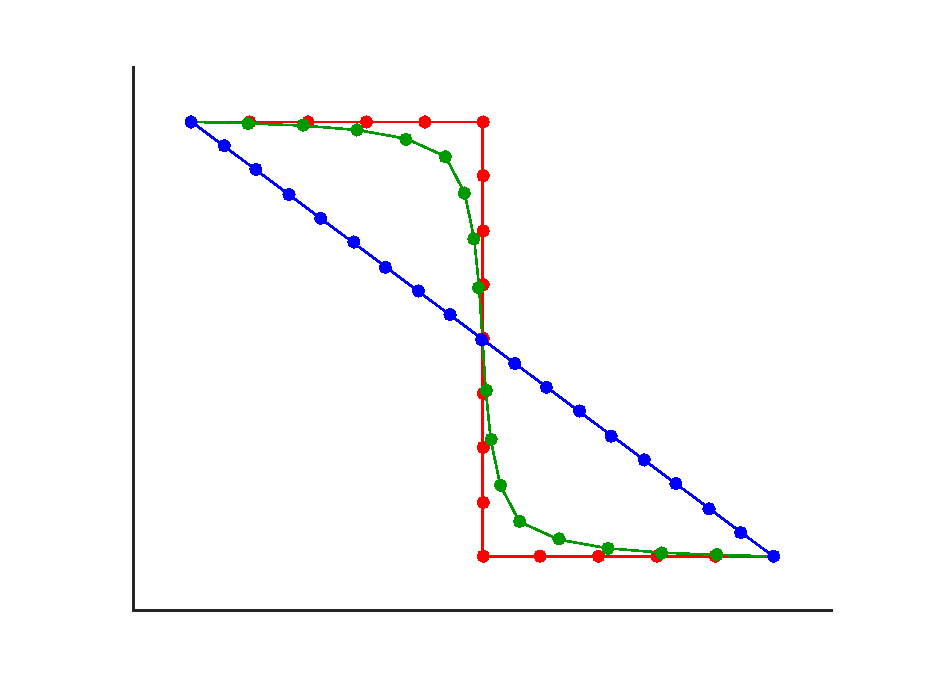
\includegraphics[width=0.5\textwidth]{Figures/Smooth.eps}
\caption{Ejemplos de suavizado}
\label{fig:Smooth}
\end{figure}

La ruta suavizada se obtiene encontrando el argumento que minimiza la función \ref{eq:Cost}, sin embargo, dada la cantidad tan grande de variables, es difícil encontrarlo analíticamente. Una forma más sencilla es mediante el médoto del descenso del gradiente, que consiste en mover el argumento pequeñas cantidades proporcionales al gradiente de la función $V$ y en sentido contrario a éste. Dado que el cambio entre cada iteración es proporcional a $\nabla V$, se puede asumir que cuando el cambio en el argumento es menor que una tolerancia, entonces se ha alcanzado el mínimo. 

El algoritmo \ref{alg:Gradient} contiene los pasos en pseudocódigo para implementar descenso del gradiente. La constante $\delta > 0$ debe ser lo suficientemente pequeña para evitar inestabilidad en el algoritmo, sin embargo, se debe considerar que entre más pequeña sea ésta, mayor será el costo computacional. 

\begin{algorithm}
\DontPrintSemicolon
\KwData{Función $V$ cuyo mínimo se desea encontrar, condición inicial $p(0)$, tolerancia $tol$.}
\KwResult{Argumento $p$ que minimiza $V$.}
$i = 0$\;
$p_i \leftarrow p(0)$\;
\While{ $\Vert\nabla V(p_i)\Vert > tol$}
{
\BlankLine
  $p_{i+1} \leftarrow p_i - \delta\nabla V(p_i)$\;
  $i \leftarrow i+1$
\BlankLine
}
Regresar $p_i$
\caption{Descenso del gradiente.}
\label{alg:Gradient}
\end{algorithm}

La ecuación \ref{eq:Cost} toma como argumentos las posiciones tanto de la ruta original como de la suavizada, sin embargo, dado que sólo varían los puntos de la nueva ruta, se puede considerar que el gradiente $\nabla V$ está dado por:
\begin{equation}
\underbrace{\left[\frac{}{}\alpha(p_1 - q_1)+\beta(p_1 - p_2)\right.}_{\ddfrac{\partial V}{\partial p_1}}
,\dots ,
\underbrace{\frac{}{}\alpha(p_i - q_i) + \beta(2p_i - p_{i-1} - p_{i+1})}_{\ddfrac{\partial V}{\partial p_i}}
,\dots ,
\underbrace{\left.\alpha(p_n-q_n)+\beta(p_n - p_{n-1})\frac{}{}\right]}_{\ddfrac{\partial V}{\partial p_n}}
\end{equation}
Nótese que se está derivando con respecto a $p$ (puntos de la ruta suavizada), no con respecto a $q$ (puntos de la ruta original). Recuerde que cada punto de la ruta tiene coordenadas $[x\,y]$, por lo que el descenso de gradiente se tiene que aplicar a ambas coordenadas. 

%%%%%
%%%%% MODELO CINEMÁTICO Y CONTROL DE POSICIÓN
%%%%%
\section{Modelo cinemático y control de posición}
\label{sec:Control}
En la sección \ref{sec:PathPlanning} se explicó el modo en que se puede calcular una ruta desde una configuración inicial hasta una final. El siguiente paso es hacer que el robot en efecto siga dicha ruta y para ello se empleará la teoría de control. 

\subsection{Modelo en variables de estado}
Para poder diseñar una ley control que haga que el robot siga la ruta deseada es necesario primero tener un modelo del robot. Para los fines de este curso, un modelo cinemático es suficiente. 

Considérese un robot diferencial como el de la figura \ref{fig:Coords} en el que la configuración está dada por tres valores $\left[x_r, y_r, \theta_r\right]$. Considerando sólo la parte cinemática y asumiendo que no existe deslizamiento en las llantas, el modelo del robot está dado por
\begin{eqnarray}                                                                                                                        
\dot{x_r} &=& \frac{v_l + v_r}{2}\cos\theta_r\label{eq:Kinematic1}\\                                                                        
\dot{y_r} &=& \frac{v_l + v_r}{2}\sin\theta_r\\                                                                                             
\dot{\theta_r} &=& \frac{v_r - v_l}{L}\label{eq:Kinematic3}                                                                               
\end{eqnarray}
donde $v_l$ y $v_r$ son las velocidades lineales de las llantas izquierda y derecha respectivamente, consideradas como señales de entrada, y $L$ es el diámetro del robot medido de eje a eje de las llantas. Se considera que el centro del robot está en el centro de dicho eje.

Nótese que no se está modelando la parte dinámica del robot, esto es, se considera que el estado del robot está dado por los mismos tres valores $\left[x_r, y_r, \theta_r\right]$ y que las velocidades de las llantas se pueden fijar de manera arbitraria. En realidad, esto no sucede así. La verdadera señal de control es el voltaje que se fija en las terminales de los motores, sin embargo, se puede considerar que las dinámicas tanto eléctrica como mecánica de dichos motores son lo suficientemente rápidas para suponer que un voltaje en el motor se reflejará \textit{rápidamente} en una velocidad angular.

\begin{figure}
\centering
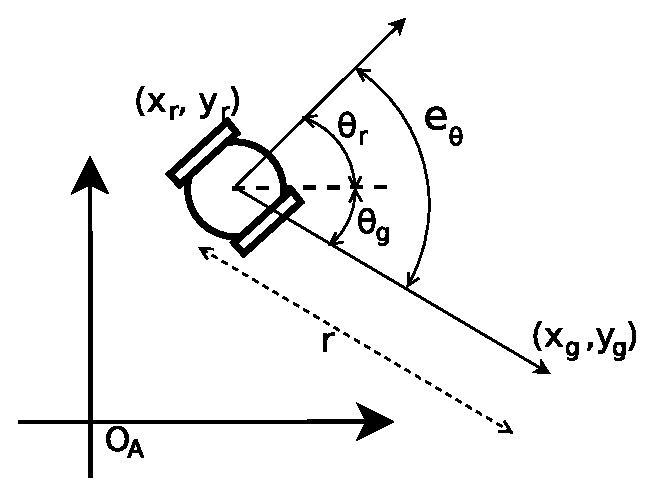
\includegraphics[width=0.5\textwidth]{Figures/GoalPose.eps}
\caption{Posición del robot y posición deseada.}
\label{fig:Coords}
\end{figure}


\subsection{Estabilidad de sistemas no lineales}
Cuando se tiene un sistema lineal invariante con el tiempo de la forma
\begin{eqnarray}
  \dot{x} &=& Ax + Bu\label{eq:SisLineal1}\\
  z &=& Cx + Du\label{eq:SisLineal2}
\end{eqnarray}
es sencillo probar su estabilidad: basta con obtener los valores propios de la matriz $A$ y si todos tienen parte real estrictamente menor que cero, entonces se puede asegurar que el sistema (\ref{eq:SisLineal1})-(\ref{eq:SisLineal2}) es exponencialmente estable, o bien, se puede obtener la función de transferencia equivalente y verificar que todas las raíces del polinomio denominador tengan parte real estrictamente negativa.

Sin embargo, el sistema dado por las ecuaciones (\ref{eq:Kinematic1})-(\ref{eq:Kinematic3}) es no lineal y por lo tanto su estabilidad no se puede analizar con las herramientas descritas en el párrafo anterior. La estabilidad en el sentido de Lyapunov o estabilidad de puntos de equilibrio es una herramienta que nos permite analizar la estabilidad de sistemas no lineales. 

Considérese un sistema dinámico de la forma 
\begin{equation}
\dot{x} = f(x) \label{eq:GeneralSystem}
\end{equation}
donde $x\in R^n$ es el vector de estados. Se dice que $x_e$ es un punto de equilibrio del sistema (\ref{eq:GeneralSystem}) si se cumple que
\begin{equation}
  \label{eq:Equilibrium}
  x(0) = x_e \implies x(t) = x_e \qquad\forall t > 0
\end{equation}
es decir, si el sistema ``comienza'' en el punto $x_e$, entonces permanece en ese punto para todo tiempo finito.

La estabilidad en el sentido de Lyapunov se define para puntos de equilibrio y existen varios tipos. Para fines de este curso sólo se utilizará la estabilidad asintótica. Suponga que se tiene un sistema de la forma (\ref{eq:GeneralSystem}) con un punto de equilibrio $x_e = 0$. Se dice que $x_e$ es asintóticamente estable, es decir, las trayectorias del sistema convergen a él conforme el tiempo tiende a infinito, si existe una función $V:R^n \rightarrow R$ tal que 
\begin{equation}
V(0) = 0 \qquad\textrm{y}\qquad V(x) > 0 \quad\forall x\neq 0 \label{eq:Lyap1}
\end{equation}
\begin{equation}
\dot{V}(x) < 0 \label{eq:Lyap2}
\end{equation}
La ecuación (\ref{eq:Lyap1}) define a $V$ como una función positivia definida, es decir, como una función escalar de variable vectorial cuyo valor es cero sólo para el vector cero, y estrictamente mayor que cero para cualquier valor diferente de cero. Esta función puede considerarse como una representación de la energía del sistema, solo que expresada en un sistema de coordenadas diferentes a las usuales. 

La equación (\ref{eq:Lyap2}) representa la variación de energía del sistema conforme pasa el tiempo y, si ésta es siempre negativa, significa que la energía siempre disminuirá y en algún momento llegará a cero, es decir, el sistema dejárá de ``moverse''. Esta derivada se tiene que evaluar a lo largo de las trayectorias del sistema (\ref{eq:GeneralSystem}). 

Nótese que se está suponiendo que el sistema tiene un punto de equilibrio en cero, sin embargo, esto no provoca pérdida de generalidad dado que cualquier punto de equilibrio se puede trasladar a cero mediante una transformación de coordenadas. Por otro lado, en la ecuación (\ref{eq:GeneralSystem}) la dinámica sólo es función de los estados y no aparecen señales de entrada, sin embargo, si se diseña un control realimentado, las señales de entrada quedarán en términos de los estados y la dinámica en lazo cerrado podrá expresarse en la forma (\ref{eq:GeneralSystem}). 

Regresando a la aplicación del robot móvil, si se quiere que el robot alcance una posición deseada, las velocidades deben ser tales que el robot tenga un punto de equilibrio asintóticamente estable en dicha posición deseada. 

\subsection{Leyes de control}
La idea del control es diseñar las señales $v_l$ y $v_r$ de modo que se garantice que el robot llegue a la posición $\left(x_g, y_g\right)$ aun en presencia de incertidumbres (como las dinámicas no modeladas) y perturbaciones. Se proponen dos leyes de control para las cuales es necesario definir primero un par de variables.

Considérese el esquema de la figura \ref{fig:Coords}. El ángulo deseado $\theta_g$ corresponde al ángulo del vector de error de posición $\left[x_g - x_r, y_g - y_r\right]$, esto es
\[\theta_g = \atantwo\left(y_g - y_r, x_g - x_r\right)\]
de donde se define el error de ángulo
\[e_{\theta} = \theta_g - \theta_r = \atantwo\left(y_g - y_r, x_g - x_r\right) - \theta_r\]
El error de distancia $r$ es simplemente la magnitud del vector de error de posición:
\[r= \left[\left(x_g - x_r\right) + \left(y_g - y_r\right)\right]^{1/2}\]
En la primera ley de control las velocidades se calculan tomando en cuenta tanto el error de posición como el de ángulo:
\begin{eqnarray}
v_{l} &=& -k_{\theta}e_{\theta} + k_d r e^{-\psi e_{\theta}^2}\label{eq:Control11}\\
v_{r} &=&  k_{\theta}e_{\theta} + k_d r e^{-\psi e_{\theta}^2}\label{eq:Control12}
\end{eqnarray}
Nótese que los primeros términos tienen igual magnitud pero signo opuesto, lo que provoca una velocidad angular que es proporcional al error de ángulo. Los segundos términos, al tener el mismo signo y misma magnitud, provocan una velocidad lineal que es proporcional al error de distancia, es decir, el robot se irá deteniendo conforme se acerque al punto meta. La exponencial sirve para hacer pequeña la velocidad lineal cuando el error de ángulo es grande, es decir, este término logra que el robot comience a avanzar hasta que esté apuntando en la dirección correcta.

En esta ley de control se tienen tres parámetros de diseño: $k_{\theta}>0$, $k_d>0$ y $\psi>0$. Las dos primeras determinan la rapidez con que el robot girará y avanzará hacia el punto meta. La tercera es muy importante. Un valor de $\psi$ muy grande hará que la velocidad lineal decrezca muy rápido cuando crece el error de ángulo, es decir, el robot comenzará a avanzar hasta que esté apuntando casi sin error hacia la meta. Por el contrario, una $\psi$ muy pequeña hará que el robot describa curvas muy grandes.  

La segunda ley de control sólo toma en cuenta el error de ángulo:
\begin{eqnarray} 
v_{l} &=& v_{max}e^{-\frac{e_{\theta}^{2}}{\alpha}} + 
\frac{D}{2}\omega_{max}\left(\frac{2}{1+e^{-\frac{e_{\theta}}{\beta}}}-1\right)\label{eq:Control21}\\
v_{r} &=& v_{max}e^{-\frac{e_{\theta}^{2}}{\alpha}} -
\frac{D}{2}\omega_{max}\left(\frac{2}{1+e^{-\frac{e_{\theta}}{\beta}}}-1\right)\label{eq:Control22}
\end{eqnarray}
En estas ecuaciones se tienen cuatro parámetros de diseño: $v_{max}$ y $\omega_{max}$ son las velocidades lineales y angulares máximas respectivamente que el robot alcanzará durante su movimiento. La constante $\alpha$ tiene una función parecida a la $\psi$ en las ecuaciones (\ref{eq:Control11})-(\ref{eq:Control12}), solo que en este caso, al estar dividiendo, una $alpha$ más pequeña provocará un descenso más pronunciado en la magnitud de la velocidad lineal. El valor de $\beta$ determina qué tanto decrece la velocidad angular conforme decrece el error de ángulo. 


%%%%%
%%%%% CAMPOS POTENCIALES ARTIFICIALES
%%%%%
\section{Campos potenciales artificiales}
En la sección \ref{sec:PathPlanning} se explicó cómo planear una ruta cuando se tiene una representación del ambiente y la seccion \ref{sec:Control} se dedicó al diseño de leyes de control que permitan seguir la ruta planeada. Sin embargo, ¿qué sucede cuando el robot tiene que evadir obstáculos que no están en el mapa y que no fueron contemplados en la planeación de la ruta? 

Un forma de evadir obstáculos es mediante campos potenciales artificiales. Una función potencial es una función real diferenciable $U: R^n \rightarrow R$ que puede verse como una función de energía y que, por lo tanto, su gradiente $\nabla U(q)$, donde $q$ es la posición del robot, representa fuerza. 

El gradiente de la función, dado por
\begin{equation}
  \label{eq:PotentialGradient}
  \nabla U(q) = \left[\frac{\partial U}{\partial q_1},\dots,\frac{\partial U}{\partial q_n}\right]
\end{equation}
es un vector que apunta en la dirección de máximo cambio de $U$. Si esta función potencial se diseña de modo que tenga un mínimo en la posición meta y máximos locales en la posición de cada obstáculo que se desee evadir, entonces se puede mover al robot mediante el algoritmo de descenso del gradiente y esto hará que el robot continúe moviéndose hasta encontrar un punto $q^*$ en el cual $\nabla U(q^*) = 0$. 

Los valores $q$ que satisfacen $\nabla U(q^*) = 0$ son llamados puntos críticos y pueden ser máximos locales, mínimos locales o puntos silla. Para determinar la naturaleza de un punto crítico, se puede utilizar la matriz Hessiana, dada por

\begin{equation}
  \label{eq:Hessian}
  H(q) = \left[
    \begin{tabular}{ccc}
      $\frac{\partial^2 U}{\partial q_1^2}$ &$ \dots$ &$ \frac{\partial^2 U}{\partial q_1 \partial q_n}$\\
      $\vdots$ & $\ddots$ & $\vdots$ \\
      $\frac{\partial^2 U}{\partial q_n\partial q_1}$ &$ \dots$ &$ \frac{\partial^2 U}{\partial q_n^2}$
    \end{tabular}
\right]
\end{equation}

Si $H(q)$ evaluada en $q^*$ es no singular, significa que $q^*$ es un punto crítico aislado. Si $H(q^*)$ es positiva definida, entonces $q^*$ es un mínimo local, si es negativa definida, se trata de un máximo local, y en otro caso, $q^*$ es un punto silla. Si $H(q^*)$ es singular, entonces significa que $q^*$ no es un punto aislado, es decir, que la función potencial $U$ es ``plana'' en la región que contiene a $q^*$. 

En general, si el robot se mueve siempre en sentido contrario al gradiente, en algún momento llegará a un mínimo local. Puede suceder que la condición inicial del robot corresponda a un máximo local o a un punto silla, en cuyo caso el robot no se moverá, pues en estos puntos el gradiente es cero. Esta situación es muy improbable, además, cualquier perturbación hará que el robot ``se mueva'' de ese punto y entonces se dirigirá al mínimo local, es decir, los puntos silla y los máximos son puntos inestables. 

\subsection{Diseño mediante campos atractivos y repulsivos}
Como se expuso previamente, la función potencial $U(q)$ debe diseñarse de modo que sea diferenciable, que tenga un mínimo en el punto meta, máximos locales en cada obstáculo, y todos sus puntos críticos deben ser aislados. Una forma sencilla de logralo es diseñando por separado dos campos: uno atractivo y otro repulsivo. La idea es que el punto meta debe generar una ``fuerza atractiva'' mientras que cada obstáculo debe generar una ``fuerza repulsiva''. 

Algunas veces no es necesario diseñar primero el campo potencial y luego obtener su gradiente, sino que se puede diseñar directamente la fuerza correspondiente al gradiente. La fuerza atractiva se debe diseñar de modo que siempre se aleje del punto meta y las fuerzas repulsivas siempre deben tener una dirección que apunte hacia el obstáculo que se desea evadir, además, las fuerzas repulsivas deben crecer conforme la distancia a dicho obstáculo disminuye y ser muy pequeñas o cero, si el robot está lo suficientemente lejos. 

Es importante recordar que las fuerzas tanto atractiva como repulsiva corresponden al gradiente de la función potencial, es decir, representan la dirección de máximo cambio, sin embargo, lo que se desea es alcanzar un mínimo, por lo que al aplicar el algoritmo de descenso del gradiente, el robot se moverá en sentido contrario a estas fuerzas. 

En este curso, la fuerza atractiva que se utilizará está dada por
\begin{equation}
  \label{eq:attractive}
  F_a = \zeta \ddfrac{\left(q - q_g\right) }{\Vert q - q_g \Vert}\qquad \zeta > 0
\end{equation}
donde $q$ es la posición actual del robot y $q_g$ es la posición a donde se desea llegar. Esta fuerza tiene una magnitud $\zeta$ constante pero su dirección apunta siempre en sentido contrario al punto meta. 

La fuerza de repulsión está dada por:
\begin{equation}
  \label{eq:repulsive}
  F_r = \begin{cases}
    \eta\left(\sqrt{\frac{1}{\Vert q_{oi} - q\Vert} - \frac{1}{d_0}}\right)\ddfrac{q_{oi} - q}{\Vert q_{oi} - q\Vert}
    & \qquad\textrm{si}\quad \Vert q_{oi} - q\Vert < d_0\\
    0 & \qquad\textrm{en otro caso}
  \end{cases}
\end{equation}
donde $q_{oi}$ es la posición del objeto $i$ y $d_0$ es una distancia de influencia tal que, si el robot está a una distancia mayor que ésta del objeto $i$, entonces la fuerza de repulsión es cero. Nótese que la magnitud de esta fuerza se incrementa conforme el robot se acerca al objeto y la raiz cuadrada produce una transición suave cuando el robot pasa por $d_0$.

La fuerza resultante se calcula como 
\begin{equation}
  \label{eq:resulting}
  F = F_a + \frac{1}{n}\sum_{i=1}^n F_r
\end{equation}
es decir, la fuerza atractiva más el promedio de las fuerzas repulsivas producidas por cada obstáculo.

Una desventaja de generar campos potenciales mediante la suma de un campo atractivo más uno repulsivo es la posibilidad de tener mínimos locales. Esto se puede solucionar con la generación de funciones potenciales mediante otros métodos como el algoritmo de \textit{wavefront}. Este algoritmo no tiene el problema de los mínimos locales pero tienen la desventaja de necesitar de una discretización del espacio.

\subsection{Movimiento por descenso del gradiente}
Una vez diseñado el campo potencial y calculado el respectivo gradiente, sólo basta con mover al robot de acuerdo con el algoritmo \ref{alg:PotFields}. La constante $\alpha > 0$ debe ser lo suficientemente pequeña para evitar oscilaciones pero sin que ello conlleve un costo computacional muy alto. 

Aunque en el algoritmo se indica que el robot seguirá moviéndose mientras la magnitud del gradiente sea mayor que cero, en una implementación real se fija una tolerancia y cuando la magnitud es menor que ésta, se detiene al robot. 
\begin{algorithm}
\DontPrintSemicolon
\KwData{Posición inicial $q_s$, posición final $q_g$, posiciones $q_{oi}$ de los obstáculos}
\KwResult{Secuencia de puntos $\{q_0,q_1, q_2, \dots\}$}
$q_0 \leftarrow q_s$\;
$i \leftarrow 0$\;
\While{$\Vert\nabla U(q_i)\Vert > 0$}
{
  $q_{i+1} \leftarrow q_i - \alpha\nabla U(q_i)$\;
  $i \leftarrow i + 1$
}
  \caption{Descenso del gradiente para mover al robot a través de un campo potencial.}
  \label{alg:PotFields}
\end{algorithm}

Finalmente, para que el robot se mueva hacia cada punto $q_i$ generado por el descenso del gradiente, se pueden utilizar las leyes de control (\ref{eq:Control21})-(\ref{eq:Control22}).

%\section{Conceptos básicos de visión computacional}

%\subsection{Espacios de color}

%\subsection{Operadores morfológicos}

%\subsection{Extracción de planos a partir de nubes de puntos} 

\section{Localización}
El problema de la localización consiste en determinar la configuración del robot dadas las lecturas de los sensores y una representación del ambiente. La localización puede ser global o local. En este curos únicamente se cubrirán dos algoritmos para localizar al robot: el Filtro de Kalman Extendido y el método del histograma. 

\subsection{El Filtro de Kalman Extendido}
El Filtro de Kalman es un algoritmo que sirve para estimar un conjunto de variables a partir de un conjunto de mediciones que contienen ruido y de un modelo del sistema cuyos procesos también contienen ruido. Este filtro puede ser considerado como un filtro bayesiano, pues la estimación de las variables es en realidad la estimación de una distribución de probabilidad conjunta dada una distribución previa y un conjunto de mediciones. 

Desde el punto de vista de la teoría de control, el Filtro de Kalman es un observador en el que la ganancia se calcula con base en las propiedades estadísticas del ruido tanto en las mediciones como en el proceso. 

El Filtro de Kalman Extendido (EKF por sus siglas en inglés) es la versión del Filtro de Kalman para sistemas no lineales. En el EKF se hace una linealización alrededor de las estimaciones actuales y se aplican los mismos pasos que se usan en sistemas lineales. 

Para realizar la estimación de la posición del robot, primero se requiere una versión discreta del modelo cinemático. Discretizando el modelo (\ref{eq:Kinematic1})-(\ref{eq:Kinematic3}), y considerando que se tiene ruido de proceso, se tiene:
\begin{eqnarray}
x_{k+1} &=& x_k + \Delta t \frac{v_l + v_r}{2}\cos\theta_k + \nu_1\label{eq:Discrete1}\\
y_{k+1} &=& y_k + \Delta t \frac{v_l + v_r}{2}\sin\theta_k + \nu_2\\
\theta_{k+1} &=& \theta_k + \Delta t \frac{v_r - v_il}{L} + \nu_3\label{eq:Discrete3}
\end{eqnarray}
donde $\Delta t$ representa el periodo de muestreo y $\nu = \left[\nu_1\;\nu_2\;\nu_3\right]^T$ es ruido gaussiano sin correlación temporal, media cero y matriz de covarianza $Q$. 

La estimación de la posición del robot por filtro de Kalman consta de los siguientes pasos:

\textbf{Predicción:} Con base en el modelo cinemático y el modelo de observación, se predice el siguiente estado y la salida considerando que el ruido es cero tanto en el modelo de transición de estados como en el modelo de obsevación:
\begin{eqnarray*}
\hat{X}(k+1|k) &=& \hat{F}(X(k|k), u(k))\\
\hat{Z}(k+1|k) &=& \hat{X}(k+1|k)\\
P(k+1|k) &=& J(k)P(k|k)J^T(k) + Q
\end{eqnarray*}
donde la matriz $P$ es la covarianza del error de estimación y $J$ es el Jacobiano de la función $F$ con respecto a $X$.

\textbf{Actualización:} Con base en el error de observación y la covarianza del error de estimación se calcula el estado siguiente estimado.
\begin{eqnarray*}
S(k+1) &=& H(k+1)P(k|k+1)H^T(k+1) + R\\
K(k+1) &=& P(k+1|k)H^T(k+1)S(k+1)^{-1}\\
\hat{X}(k+1|k+1) &=& \hat{X}(k+1|k) + K(k+1)(Z(k+1) - \hat{Z}(k+1|k))\\
P(k+1|k+1) &=& (I-P(k+1)H(k+1))P(k+1|k)
\end{eqnarray*}
donde $H$ es el Jacobiano del modelo de observación, que en este caso es la identidad dado que se considera que se mide el estado completo del robot. La matriz $K$ es conocida como ganancia de Kalman.


\subsection{Método del histograma}
La localización por el método de histograma permite estimar la posición del robot con base en observaciones del ambiente pero tomando en cuenta las probabilidades de error tanto en la observación como en el movimiento. Se asume que el robot sólo puede estar en configuraciones discretas bien definidas por lo que el método es factible sólo cuando se tienen pocos grados de libertad, como en el caso del robot diferencial que se mueve sólo en un plano. 

Considere la posición del robot como un variable aleatoria discreta $X$ que puede tomar los valores $x_i=\{x_1 \dots x_n\}$ y las observaciones que puede realizar el robot como otra variable aleatoria $O$ con posibles valores $o_i=\{o_1 \dots o_m\}$. Las observaciones del robot pueden ser cualquier tipo de \textit{marca} que se pueda extraer a partir de la información de los sensores. 

Se asume que la posición inicial se desconoce por completo, por lo que el primer paso es asignar a cada posición la misma probabilidad
\begin{equation}
P(x_i) = \ddfrac{1}{n}
\end{equation}
es decir, inicialmente se tiene una distribución uniforme que indica total incertidumbre sobre la posición actual del robot. El objetivo es construir una función de densidad de probabilidad que, conforme el robot se mueva y realice observaciones, tienda hacia una distribución unimodal cuyo máximo indique la posición actual del robot.

\textbf{Observación.} 

Para comenzar a estimar la posición del robot es necesario realizar observaciones el ambiente. Para ello, a cada nodo $v$ del grafo $G$ se le asigna una marca que ``debería'' ser observada si el robot se encontrara en ese nodo. 

Con cada observación se debe modificar la probabilidad de cada nodo, dado que se identificó determinada marca. Considérese la posición del robot como una variable aleatoria $V$ que puede tomar los valores $v_i =\left\{\textrm{entrada-izquierda, sala-frente,...}\right\}$ y sea $O = \{o_j\}$ la variable aleatoria que representa la marca observada.


Una vez hecha una observación, se desea actualizar la probabilidad de cada nodo $v_i$, dada la observación $o_j$, esto es
\begin{equation}
P(V = v_i| O = o_j)
\end{equation}
que de acuerdo con el teorema de Bayes se puede calcular como
\begin{equation}
P(v_i| o_j) = \frac{P\left(o_j|v_i\right)P\left(v_i\right)}{P\left(o_j\right)}
\end{equation}
En la ecuación anterior, el término $P\left(o_j|v_i\right)$ es la probabilidad  de que se  observe una determinada marca si se asume que el robot está en el nodo $v_i$, es decir, la probabilidad de $o_j$ en la hipótesis $v_i$. Esta probabilidad se calcula de forma estadística en la etapa de entrenamiento. Si se observa la marca $o_j$ existen dos posibles casos: que la marca corresponda al nodo en el que se asume el robot se encuentra o, que no corresponda. Llamaremos al primer caso un acierto verdadero (AV), y al segundo, un falso positivo (FP). En este trabajo se consideraron las probabilidades
\begin{eqnarray}
P(AV)&=&0.6\\
P(FP)&=&0.25
\end{eqnarray}
El término $P\left(v_i\right)$ denota la probabilidad a priori del nodo $v_i$ y el término $P\left(o_j\right)$ puede calcularse, de acuerdo con el teorema de la probabilidad total, como
\begin{equation}
P\left(o_j\right) = \sum_i^n P\left(o_j|v_i\right)P\left(v_i\right)
\end{equation}
donde $n$ es el número total de nodos del grafo $G$ que representa el ambiente. 

\textbf{Movimiento}
Como se explicó anteriormente, se asume que el robot puede ejecutar tres movimientos: frente, izquierda y derecha. Para modelar la incertidumbre en el movimiento, se asume que existen dos posibles casos: el robot alcanza el nodo deseado o, el robot se queda en el nodo en que ya estaba. Llamaremos al primer caso movimiento correcto (MC) y al segundo, movimiento con falla (MF). Al igual que en el modelo de observación, las probabilidades de ambos casos se calcularon mediante experimentos en la etapa de entrenamiento. Los valores usados fueron:
\begin{eqnarray}
P(MC) &=& 0.7\\
P(MF) &=& 0.3
\end{eqnarray}
Para calcular la probabilidad de cada nodo después de un movimiento, se usa nuevamente el teorema de la probabilidad total. La probabilidad a posteriori de un nodo $v_i$ es la probabilidad de que el robot haya llegado a ese nodo por un movimiento correcto o bien, por un movimiento con falla, es decir
\begin{equation}
P\left(v_i^t\right) = \sum_k P\left(v_i^t|v_k^{t-1}\right) P\left(v_k^{t-1}\right)
\end{equation}
donde los superíndices $t$ y $t-1$ indican el tiempo actual y el tiempo anterior, respectivamente. Si se considera que el robot solo puede llegar a un nodo por un movimiento correcto (viniendo desde otro nodo) o por uno con falla (el robot permanece en el mismo nodo), entonces la ecuación se puede escribir como
\begin{equation}
P\left(v_i^t\right) = P\left(v_i^t|v_k^{t-1}\right)P\left(v_k^{t-1}\right) + P\left(v_i^t|v_i^{t-1}\right)P\left(v_i^{t-1}\right)
\end{equation}
El término $P\left(v_i^t|v_k^{t-1}\right)$ indica la probabilidad de que el robot llegue al nodo $v_i$ desde el nodo $v_k$ (un movimiento correcto), es decir
\begin{equation}
P\left(v_i^t|v_k^{t-1}\right) = P(MC)
\end{equation}
y de modo similar
\begin{equation}
P\left(v_i^t|v_i^{t-1}\right) = P(MF)
\end{equation}


\section{La plataforma ROS}

\bibliography{References}
\end{document}
%%% Local Variables:
%%% mode: latex
%%% TeX-master: t
%%% End:
